% ----------------------------------------------------------
% Arquivo de configuração do documento (provido pelo template)
% ----------------------------------------------------------
%-------------------------------------------------------------------------
% Modelo Trabalho PPGE-UFPB/Estatística
% Normas da ABNT
% Provedor: Laboratório de Economia e Modelagem Aplicada -- LEMA
%-------------------------------------------------------------------------

\documentclass[12pt, oneside, a4paper, english, brazil]{abntex2}

% ----------------------------
% Pacotes básicos 
% ----------------------------
% Referências
\usepackage[brazilian,hyperpageref]{}	
\usepackage[alf]{abntex2cite}			

% Texto aleatório (para testes)
\usepackage{lipsum} 

% Fonte e codificação (acentuação)
\usepackage{lmodern}       
\renewcommand{\sfdefault}{ppl}
\usepackage[T1]{fontenc}	
\usepackage[utf8]{inputenc}	

\usepackage{tocloft}
\usepackage{array}


\usepackage{array}     % Necessário para >{\centering\arraybackslash}
\usepackage{booktabs}  % Para \toprule, \midrule, \bottomrule
\usepackage{float}     % Para [H] no ambiente table



% Tabelas e Figuras
\usepackage{ctable}             
\usepackage{multirow}
\usepackage{array}
\usepackage{float}              
\usepackage{longtable}          
\usepackage{xcolor,colortbl}    
\usepackage{booktabs}           
\usepackage{graphicx}			
\usepackage{subfig}             
\usepackage{caption}            
\usepackage{epstopdf}           

% Equações e símbolos
\usepackage{amsmath}            
\usepackage{nomencl} 
\usepackage{cleveref}  

% Texto
\usepackage{indentfirst}		
\usepackage{color}				
\usepackage{microtype} 			
\usepackage{lastpage}			

% ----------------------------------------------------------
% Configurações do texto
% ----------------------------------------------------------

\usepackage{array}
\newcolumntype{L}[1]{>{\raggedright\let\newline\\\arraybackslash\hspace{0pt}}m{#1}}
\newcolumntype{C}[1]{>{\centering\let\newline\\\arraybackslash\hspace{0pt}}m{#1}}
\newcolumntype{R}[1]{>{\raggedleft\let\newline\\\arraybackslash\hspace{0pt}}m{#1}}

\makeatletter
\hypersetup{
  pdftitle={\@title}, 
  pdfauthor={\@author}
}
\makeatother

% ----------------
% Informe os dados
% ----------------
\local{João Pessoa - PB}
\data{\the\year}

\instituicao{
	Universidade Federal da Paraíba 
	\par
	Centro de Ciências Sociais Aplicadas
	\par
	Programa de Pós-Graduação em Economia}
\tipotrabalho{Projeto de Disciplina}

\preambulo{
  Trabalho apresentado ao Programa de Pós-Graduação em Economia da Universidade Federal da Paraíba, em cumprimento às exigências da disciplina de \disciplina, ministrada pelo professor Dr. \professor.
}

%--------------------------------------------------------------
% Recuo ABNT
%--------------------------------------------------------------
\newcommand\parindentABNT{
  \setlength{\parindent}{1.25cm} 
  \setlength{\parskip}{0.1cm} 
}

%--------------------------------------------------------------
% Redefinir \chapter: alinhado à esquerda, letras normais, tamanho \large
%--------------------------------------------------------------
\makeatletter
% Capítulos com número (\chapter{})
\renewcommand{\@makechapterhead}[1]{%
  \vspace{2cm}%
  {\centering
   \Large\ABNTEXchapterfont\bfseries
   \thechapter\quad #1\par
  }%
  \vspace{1cm}%
}
% Capítulos sem número (\chapter*{})
\renewcommand{\@makeschapterhead}[1]{%
  \vspace{2cm}%
  {\centering
   \Large\ABNTEXchapterfont\bfseries
   #1\par
  }%
  \vspace{1cm}%
}
\makeatother









% --- PACOTES DE FORMATAÇÃO ADICIONAL ---
\usepackage{caption}
\usepackage{float} % Pacote para forçar o posicionamento de figuras com [H]
\captionsetup{
  justification=raggedright, % Alinha à esquerda.
  singlelinecheck=false,     % Remove a verificação de uma única linha para manter o alinhamento.
  font={bf,small} 
  }

% --- CONTADORES PARA CAPÍTULOS E SEÇÕES MANUAIS ---
\newcounter{manualchapter}
\setcounter{manualchapter}{0}

\newcounter{manualsection}[manualchapter] % Cria o contador de seção, resetado por capítulo
\renewcommand{\themanualsection}{\themanualchapter.\arabic{manualsection}} % Define o formato (ex: 2.1)
% --- FIM DO BLOCO ---


% ----------------------------------------------------------
% Metadados do trabalho
% ----------------------------------------------------------
\titulo{Desistência em Cursos no Ensino Superior Público Federal Brasileiro: Uma Análise de 2018 a 2023 com Técnicas de Machine Learning}
\autor{Elton John Marinho de Lima}
\newcommand\disciplina{Estatística}
\newcommand\professor{Aléssio Tony C. Almeida}

% ----------------------------------------------------------
% Estilo de página personalizado: só número no topo direito
% ----------------------------------------------------------
\usepackage{fancyhdr}
\fancypagestyle{somenteNumero}{
  \fancyhf{}  % limpa tudo
  \fancyhead[R]{\thepage}  % número no canto superior direito
  \renewcommand{\headrulewidth}{0pt}  % sem linha no topo
}

% -------------------------------
% Alinhamento do sumário no abntex2
% -------------------------------
\makeatletter
% Seção (nível 1)
\renewcommand{\l@section}[2]{%
  \@dottedtocline{1}{0em}{5.15em}{#1}{#2}}

% Subseção (nível 2)
\renewcommand{\l@subsection}[2]{%
  \@dottedtocline{2}{10.3em}{3.2em}{#1}{#2}}
\makeatother

% -----------------------------------------------
% Alinhar título de capítulo à esquerda, menor e em negrito — abntex2
% -----------------------------------------------
% Deixar títulos de capítulo em negrito, menor e alinhados à esquerda (abntex2)
\renewcommand{\ABNTEXchapterfont}{\bfseries\normalsize}
\renewcommand{\ABNTEXchapterfontsize}{\normalsize}

\makeatletter
\renewcommand{\bibsection}{%
  \addcontentsline{toc}{chapter}{Referências}% Adiciona ao sumário
  \vspace{2em}%
  \noindent\normalsize\textbf{Referências}%
  \vspace{1em}\par
    \normalsize % Tamanho 12pt
}
\makeatother

\makeatletter
\renewcommand{\tableofcontents}{%
  \vspace{2em}%
  \noindent\normalsize\textbf{Sumário}%
  \vspace{1em}\par
  \normalsize
  \@starttoc{toc}%
}
\makeatother


\newcommand{\espacoentreparagrafos}{
  \par\vspace{0.5cm}\noindent\hspace{1.25cm}
}


% ----------------------------------------------------------
% Início do documento
% ----------------------------------------------------------
\begin{document}

% Gera a capa, folha de rosto, etc.
% ----------------------------------------------------------
% Elementos pré-textuais
% ----------------------------------------------------------
\pretextual


%---------------------------------------------------
% CAPA, CONTRACAPA E FICHA CATALOGRÁFICA 
%---------------------------------------------------


%---------------------------------------------------
% Capa
%\imprimircapa MODELO ABNT GERAL 
% Modelo personalizado abaixo
%---------------------------------------------------

\setlength{\parindent}{0cm}
\chapter*[capa]{}
\begin{minipage}{\linewidth}
	
	\centering
	
	\begin{tabular}{cl}
		\begin{minipage}{0.35\textwidth}
			\centering	
\includegraphics[scale=0.15]{config/logo-ppge}
		\end{minipage}
		&
		\begin{minipage}{1\textwidth}
			%\centering
			\large\ABNTEXchapterfont\SingleSpacing{
			\imprimirinstituicao
			\vspace{5mm}
		}
		\end{minipage}
	\\	
	\end{tabular} 	
	
\end{minipage}

%		\begin{minipage}{0.75\textwidth}
%	
%		
%		\imprimirinstituicao
%		
%		\vspace{5mm}
%	}
%\end{minipage}


				



\vfill

	\begin{minipage}{\linewidth}
	\begin{center}
		{\large\ABNTEXchapterfont\SingleSpacing\bfseries
			
         \centering   \imprimirtitulo
		}
	\end{center}
	
	\begin{flushright}
		\begin{minipage}{10cm}
			\SingleSpacing
			\imprimirpreambulo
		\end{minipage}
	\end{flushright}
	
		
		
\end{minipage}


\vfill

\begin{center}
	\begin{minipage}{\linewidth}
		\centering\large\ABNTEXchapterfont\SingleSpacing {
			
     	\imprimirautor
		
		
		}
	\end{minipage}
\end{center}


\vfill

\begin{center}
	\begin{minipage}{\linewidth}
		\centering\normalsize\ABNTEXchapterfont\SingleSpacing {
			\imprimirlocal \\ \imprimirdata
		}
	\end{minipage}
	
	
\end{center}



\cleardoublepage

\newpage

\makeatother

% -------------------------------
% Inserir o sumário
% -------------------------------
\pdfbookmark[0]{\contentsname}{toc}
\tableofcontents*
\cleardoublepage









% --- SEÇÃO MANUAL DE RESUMO E ABSTRACT NA MESMA PÁGINA ---
\pdfbookmark[0]{Resumo}{resumo} % Adiciona o marcador no PDF
\thispagestyle{empty} % Remove cabeçalho e rodapé desta página

\noindent
\textbf{Resumo}

\vspace{1em} % Espaçamento vertical

\noindent
A desistência no ensino superior representa um desafio significativo para as instituições públicas federais, com profundos impactos econômicos e sociais. Este estudo analisa o fenômeno em cursos de graduação de Instituições Federais de Ensino Superior (IFES) no Brasil, de 2018 a 2023, a partir da integração de microdados do INEP e da RAIS. Utilizando um modelo de machine learning (Random Forest), identificaram-se os principais fatores preditivos e as características associadas às altas taxas de desistência. Os resultados indicam que indicadores de qualidade institucional, como o IGC e o CPC, são os preditores de maior influência, superando fatores isolados de desempenho discente. O modelo demonstrou desempenho robusto, com alta acurácia e capacidade de generalização, validado por múltiplas métricas de performance. O trabalho contribui para a literatura ao aplicar uma abordagem preditiva ao tema e, do ponto de vista social, oferece subsídios para que gestores formulem políticas de permanência mais eficazes e direcionadas.

\vspace{1em}

\noindent
\textbf{Palavras-chave}: Desistência Universitária. Ensino Superior. Instituições Federais. Machine Learning. Fatores Preditivos. Políticas de Permanência.

\vspace{3em} % Espaço maior entre o resumo e o abstract

\noindent
\textbf{Abstract}

\vspace{1em}

\noindent
Dropout in higher education represents a significant challenge for federal public institutions in Brazil, with profound economic and social impacts. This study analyzes this phenomenon in undergraduate courses at Brazilian Federal Higher Education Institutions (IFES) from 2018 to 2023, by integrating microdata from INEP and RAIS. Using a machine learning model (Random Forest), the main predictive factors and characteristics associated with high dropout rates were identified. The results indicate that institutional quality indicators, such as the IGC and CPC, are the most influential predictors, outweighing isolated factors of student performance. The model demonstrated robust performance with high accuracy and generalization capacity, validated by multiple performance metrics. This work contributes to the literature by applying a predictive approach to the topic and, from a social standpoint, offers strategic insights for managers and policymakers to formulate more effective and targeted retention policies.

\vspace{1em}

\noindent
\textbf{Keywords}: University Dropout. Higher Education. Federal Universities; Machine Learning; Predictive Factors; Retention Policies.

% --- FIM DA SEÇÃO MANUAL ---


% --- Início da parte textual ---
\textual
\parindentABNT
\clearpage % Força o início do conteúdo textual em uma nova página

% ----------------------------------------------------------
% Sumário com número no canto superior direito, sem "SUMÁRIO"
% ----------------------------------------------------------
\pagestyle{somenteNumero}
\pdfbookmark[0]{\contentsname}{toc}
\cleardoublepage


% --- CAPÍTULO MANUAL: Introdução ---
\refstepcounter{manualchapter}
\addcontentsline{toc}{chapter}
{\protect\numberline{\themanualchapter}Introdução}
\vspace{2em}
\noindent\textbf{\themanualchapter. Introdução}
\vspace{1em}
\par

As instituições de ensino superior públicas federais contribuem significativamente para o desenvolvimento educacional e profissional no Brasil. Em um cenário no qual o mercado de trabalho demanda crescente qualificação, tais instituições promovem o acesso ao conhecimento, à pesquisa e à inovação, desempenhando, assim, um papel estratégico na formação de cidadãos capacitados para os desafios socioeconômicos do país. Contudo, apesar dos esforços direcionados a garantir o acesso e a permanência discente, a desistência nos cursos de graduação emerge como um dos principais obstáculos à efetividade dessas políticas educacionais \cite{santos2024previsao}.

A desistência nos cursos das instituições de ensino superior (IES) públicas federais tem sido um desafio para a educação brasileira. O fenômeno, caracterizado pelo abandono do curso pelo discente antes de sua conclusão, não é recente. Tal questão tem despertado atenção governamental desde meados de 1995, quando foi instituída pelo Ministério da Educação a Comissão Especial de Estudos sobre o Abandono Estudantil. Essa pauta é de grande interesse, pois o abandono acarreta não apenas impactos negativos ao sistema educacional, mas também expressivas perdas econômicas, uma vez que onera o orçamento das IES \cite{pinheiro2018}.

O presente estudo tem como objetivo analisar a desistência em cursos de graduação de instituições federais de ensino superior. Para tanto, serão utilizadas as bases de dados do Instituto Nacional de Estudos e Pesquisas Educacionais Anísio Teixeira (INEP) e do Ministério do Trabalho e Emprego (MTE), especificamente os microdados dos Indicadores de Qualidade da Educação Superior e da Relação Anual de Informações Sociais (RAIS), compreendendo o período de 2018 a 2023. Nesse sentido, a pesquisa busca responder às seguintes questões: Quais variáveis socioeconômicas e institucionais têm maior impacto sobre a desistência do discente nas universidades públicas federais? Dentre os cursos ofertados, existem características intrínsecas que se mostram determinantes para as elevadas taxas de desistência?

O objetivo principal desta pesquisa é identificar os fatores determinantes da desistência em cursos de IES públicas federais por meio da aplicação de um modelo de machine learning. Este propósito se desdobra em dois objetivos específicos: Identificar e analisar as variáveis de maior impacto associadas ao fenômeno da desistência dos discentes; e avaliar a performance do algoritmo Random Forest, um modelo de aprendizagem supervisionada, na predição da desistência, mensurando sua acurácia e utilizando sua capacidade de inferência para interpretar os fatores mais relevantes.

\newpage

A contribuição acadêmica deste estudo reside na aplicação de técnicas de machine learning para a análise da desistência no ensino superior, uma abordagem ainda incipiente na literatura educacional brasileira. Ao integrar métodos preditivos avançados à análise de dados institucionais, a pesquisa inova nas abordagens metodológicas aplicadas ao estudo da permanência discente e oferece uma base empírica mais robusta para a identificação de padrões e variáveis de risco. Do ponto de vista social, a pesquisa contribui ao fornecer subsídios para que gestores públicos e institucionais possam elaborar políticas de apoio mais eficazes. Tais políticas, informadas por evidências, são essenciais para orientar ações preventivas, visando não apenas à redução dos índices de desistência, mas também à promoção da equidade no acesso e na conclusão do ensino superior.

Este trabalho está estruturado em seis seções. A primeira apresenta a fundamentação teórica da pesquisa por meio de uma revisão da literatura pertinente. A segunda seção detalha a metodologia empregada. A terceira descreve a base de dados e as técnicas de pré-processamento utilizadas. A quarta realiza uma análise descritiva dos dados. A quinta apresenta e discute os resultados obtidos na análise. Por fim, a sexta seção expõe as considerações finais, sintetizando as conclusões e as implicações do estudo.

% --- CAPÍTULO MANUAL: Referencial Teórico ---
\refstepcounter{manualchapter}
\addcontentsline{toc}{chapter}{\protect\numberline{\themanualchapter}Referencial Teórico}
\vspace{2em}
\noindent\textbf{\themanualchapter. Referencial Teórico}
\vspace{1em}
\par

O fenômeno do abandono estudantil constitui um campo de estudo consolidado no meio acadêmico, com inúmeras pesquisas dedicadas a essa temática. Esta seção apresenta uma revisão da literatura recente e está organizada em dois subtópicos principais.

O primeiro, intitulado "Desistência no Ensino Superior: Conceitos, Causas e Impactos", explora os fatores sociais, econômicos e institucionais associados ao fenômeno. O segundo, "Aplicação de Machine Learning na Educação", discute o uso de métodos preditivos, com foco em algoritmos como o Random Forest, para a análise da desistência.

% --- SEÇÃO MANUAL: Exemplo 1 ---
\refstepcounter{manualsection}
\addcontentsline{toc}{section}{\protect\numberline{\themanualsection}Desistência no ensino superior: conceitos, causas e impactos}
\vspace{1.5em}
\noindent\textbf{\themanualsection\hspace{1em}Desistência no ensino superior: conceitos, causas e impactos}
\vspace{0.5em}
\par

De acordo com o Instituto Nacional de Estudos e Pesquisas Educacionais Anísio Teixeira (INEP), o conceito de desistência se aplica à situação em que o discente tem seu vínculo com o curso de origem formalmente encerrado, o que é registrado por meio do status de "desvinculado" ou "transferido para outro curso da mesma IES" \cite{inep2017}.

A prevalência da desistência discente no ensino superior suscita questionamentos fundamentais para a gestão acadêmica e para as políticas educacionais. Nesse contexto, torna-se imperativo investigar as múltiplas facetas desse problema: Quais são os principais fatores que levam os discentes a abandonar seus cursos? Quais os impactos resultantes desse fenômeno para os programas de graduação e para as próprias instituições? Adicionalmente, é crucial analisar quais estratégias as IES têm implementado para mitigar as taxas de desistência e, em uma perspectiva mais ampla, em que medida a persistência desse desafio compromete a eficácia e o cumprimento da missão social da universidade.

A finalidade do ensino superior público brasileiro transcende a simples formação de mão de obra. A Lei de Diretrizes e Bases da Educação Nacional (LDB), Lei nº 9.394/1996, estabelece em seu capítulo IV as normas que regulamentam essa modalidade de ensino \cite{brasil1996}. Nesse escopo, as Instituições de Ensino Superior (IES) não se limitam a conceder diplomas; elas têm o papel fundamental de contribuir para o desenvolvimento de uma sociedade mais justa, democrática e plural. Conforme apontam \citeonline{coimbra2021}, essa missão se concretiza por meio da promoção articulada do ensino, da pesquisa científica e da extensão. Esse tripé universitário busca fomentar a participação ativa tanto dos discentes quanto da comunidade em geral.

O problema da desistência estudantil não se restringe às instituições de ensino superior públicas, configurando-se como um fenômeno de âmbito geral que afeta também o setor privado. As causas para esse fenômeno são frequentemente categorizadas em dois eixos: fatores internos, de natureza institucional, e fatores externos, de ordem socioeconômica.

De acordo com \citeonline{soares2020}, entre os principais fatores internos destacam-se a infraestrutura institucional inadequada, o apoio pedagógico deficitário e a baixa qualidade do ensino. No âmbito dos fatores externos, o autor aponta questões sociais, como a falta de incentivo familiar, e dificuldades econômicas, que incluem os desafios financeiros durante o curso e a complexa conciliação com as demandas do mercado de trabalho.

Os impactos da desistência, tanto para a instituição quanto para a sociedade, podem ser entendidos como desperdícios de ordem social, acadêmica e econômica. Conforme \citeonline{santos2024evasao}, quando um discente de universidade pública desiste de seu curso, o investimento estatal alocado em sua vaga é perdido, uma vez que os recursos financeiros planejados não geram o retorno esperado.

Essa subutilização acarreta a ociosidade de toda a infraestrutura de apoio, incluindo o corpo docente, os equipamentos postos à disposição, os espaços físicos e o corpo técnico-administrativo mobilizado para atender às demandas do curso.

Diante desse cenário, a fim de mitigar as perdas associadas à desistência, torna-se estratégico que gestores e tomadores de decisão implementem mecanismos preditivos. A aplicação de ferramentas como o Machine Learning é fundamental para a detecção precoce de discentes com risco de desistência, possibilitando um direcionamento mais eficaz de recursos para ações preventivas. Consequentemente, essa abordagem otimiza o uso do orçamento público e minimiza os desperdícios.

A próxima seção aborda a aplicação de machine learning na educação, com foco em estudos que têm utilizado essa abordagem para identificar os fatores associados à desistência no ensino superior. Será demonstrado como essa técnica pode ser empregada para analisar e compreender as causas desse fenômeno.

% --- SEÇÃO MANUAL: Exemplo 2 ---
\refstepcounter{manualsection}
\addcontentsline{toc}{section}{\protect\numberline{\themanualsection}Aplicação de machine learning para identificação de causas de desistências no ensino superior}
\vspace{1.5em}
\noindent\textbf{\themanualsection\hspace{1em}Aplicação de machine learning para identificação de causas de desistências no ensino superior}
\vspace{0.5em}
\par

O Machine Learning (ML), ou Aprendizado de Máquina, é conhecido como um campo da Inteligência Artificial no qual algoritmos aprendem padrões diretamente dos dados de forma automática. Com base nesse aprendizado, os sistemas realizam tarefas como predição ou classificação por meio de modelos, que podem ser supervisionados ou não supervisionados.

No aprendizado supervisionado, o modelo é treinado com um conjunto de dados que já inclui a variável de resultado (a variável "explicada"). Utilizando um conjunto de variáveis explicativas, o algoritmo aprende a mapear a relação entre elas e o resultado, tornando-se capaz de fazer previsões de forma eficiente para novas observações.

Essa abordagem metodológica tem se mostrado eficaz na área da educação. Conforme \citeonline{pinheiro2018}, sua aplicação permite identificar com alta precisão os principais fatores associados à desistência por parte dos discentes, contribuindo para a análise do fenômeno.

Diversos autores têm utilizado algoritmos de aprendizado supervisionado como Random Forest (RF) para modelar o fenômeno da desistência universitária.

Estudos recentes, por exemplo, empregam técnicas como Logistic Regression, Gradient Boosting, XGBoost e o próprio Random Forest para realizar previsões a partir de bases de dados públicas. Nesse contexto, \citeonline{malerba2023} relata que modelos baseados em árvores de decisão, como o Random Forest e o Decision Tree, podem alcançar uma precisão superior a 90\% na identificação de discentes com risco de desistência.

O objetivo deste estudo é identificar os principais fatores associados à desistência em universidades públicas federais brasileiras. Para tal, será aplicado o algoritmo de machine learning Random Forest a um conjunto de dados socioeconômicos e de indicadores da qualidade do ensino superior.

A metodologia de pesquisa, com os detalhes sobre o modelo empregado, é apresentada na Seção 3. Por sua vez, a Seção 4 é dedicada à descrição da base de dados e aos procedimentos de pré-processamento aplicados.


% --- CAPÍTULO MANUAL: Metodologia ---
\refstepcounter{manualchapter}
\addcontentsline{toc}{chapter}{\protect\numberline{\themanualchapter}Metodologia}
\vspace{2em}
\noindent\textbf{\themanualchapter. Metodologia}
\vspace{1em}
\par

Nesta pesquisa, será realizada uma análise preditiva da desistência por meio de um modelo de aprendizado supervisionado, utilizando o algoritmo Random Forest. A análise cobrirá o período de 2018 a 2023.

A variável-alvo (explicada) do modelo é a taxa de desistência acumulada de cada curso. Para a tarefa de classificação, essa variável contínua foi convertida em uma variável binária, utilizando a mediana da distribuição como ponto de corte: 1: Alta taxa de desistência (valores acima da mediana); 0: Baixa taxa de desistência (valores iguais ou inferiores à mediana).

Para garantir a consistência temporal, todos os dados foram agregados como a média do período em análise (2018-2023). As variáveis explicativas do modelo serão compostas por três grupos de indicadores:
\begin{enumerate}
    \item Indicadores de Qualidade: Métricas que avaliam a excelência de cada curso.
    \item Variável de Porte do Curso: A quantidade de vagas ofertadas, utilizada como uma medida de sua dimensão.
    \item Variável Socioeconômica: O salário médio de mercado para os profissionais formados na respectiva área.
\end{enumerate}

A relação entre essas variáveis no modelo pode ser formalizada da seguinte maneira:
\begin{multline}
    D_{acum_{t+5}} = \alpha_{i} + \beta_{1}X_{idd.pad.} + \beta_{2}X_{org.did.ped.} + \beta_{3}X_{infra.} + \beta_{4}X_{op.ampl.form.} \\
    + \beta_{5}X_{n.mestres} + \beta_{6}X_{n.doutores} + \beta_{7}X_{c.enade} + \beta_{8}X_{id.cont.} + \beta_{9}X_{c.grad.} \\
    + \beta_{10}X_{igc} + \beta_{11}X_{sal.} + \beta_{12}X_{v.ofert.} + \epsilon_{i}
\end{multline}

A variável explicada: $D_{acum_{t+5}}$ formada pela taxa de desistência acumulada no tempo $t+5$. As variáveis explicativas são: $X_{idd.pad.}$ nota padronizada do Indicador de Diferença entre os Desempenhos Observado e Esperado (IDD), $X_{org.did.ped}$ nota padronizada da organização didático-pedagógica do curso, $X_{infra.}$ nota padronizada da infraestrutura e das instalações físicas, $X_{op.ampl.form}$ nota padronizada referente à oportunidade de ampliação da formação, $X_{n.mestres}$ nota padronizada do percentual de professores com titulação de mestrado, $X_{n.doutores}$ nota padronizada do percentual de professores com titulação de doutorado, $X_{c.enade}$ conceito Enade contínuo, $X_{idd.cont.}$ Indicador de Diferença entre os Desempenhos Observado e Esperado (IDD) contínuo, $X_{c.grad}$ Conceito Preliminar de Curso (CPC) contínuo, $X_{igc}$ Índice Geral de Cursos (IGC) contínuo da instituição, $X_{sal}$ média salarial da área de formação do curso, $X_{v.ofert.}$ número de vagas ofertadas pelo curso e $\epsilon_{i}$ erro residual do modelo, que captura os fatores não observados que influenciam a variável dependente.

Segundo \citeonline{morettin2022}, o Random Forest é um método de ensemble que constrói múltiplas árvores de decisão e combina suas predições para gerar um resultado final mais robusto e preciso. Para tarefas de regressão, essa combinação geralmente corresponde à média das previsões de cada árvore, visando minimizar o erro quadrático médio (MSE), enquanto para classificação, o resultado é determinado pela classe mais votada.

\newpage

De acordo com \citeonline{james2023}, o modelo Random Forest constrói um conjunto de árvores de decisão (T). Cada árvore individual (t) é treinada com base em uma amostra de bootstrap (reamostragem com reposição) dos dados e, em cada nó, a divisão considera apenas um subconjunto aleatório das variáveis disponíveis.

A previsão final para uma nova observação (x) é então obtida pela agregação das predições de todas as árvores. O resultado é a média das previsões individuais, conforme representado pela seguinte função:
$$ \hat{Y}_{RF}(x) = \frac{1}{T}\sum_{t=1}^{T}\hat{Y}_{t}(x) $$
Onde $\hat{y}_{t}(x)$ é a previsão da t-ésima árvore de decisão para a observação x.

A função objetivo que a Random Forest implicitamente tenta minimizar durante seu treinamento através da construção e combinação de árvores, do qual pode ser pensada como minimização do erro de predição médio sobre o conjunto de dados, conforme função objeto:
$$ \text{Minimizar } J_{RF}(0) = \frac{1}{N} \sum_{i=1}^{N} (y_i - \hat{Y}_{RF}(x_i))^2 $$

Do qual N é o número de observações no conjunto de dados, $y_{i}$ é o valor real da i-ésima observação, $\hat{y}_{RF}(x_{i})$ refere-se ao valor previsto pela Random Forest.

Para realizar a classificação, a função objetivo realiza a minimização do índice de Gini em cada nó da árvore durante o treinamento, e a previsão final da Random Forest seria a classe mais votada.

Para otimização da Random Forest, foi utilizado o método RFE-CV, do qual é um procedimento para encontrar o melhor subconjunto de características ótimas para compor o modelo no conjunto de validação cruzada, sendo o conjunto de características:
$$ F=\{F_{1},F_{2},...,F_{D}\} $$

Onde D é o número total de caraterísticas. A RFE-CV começa com as D características, realiza a interação, treinando a Random Forest com o conjunto de características selecionada, avalia o desempenho do modelo, classifica as características mais importantes e remove a de menor importância, repete os passos citados. Sendo que o objetivo da RFE-CV é encontrar o subconjunto de características $F^{*}\subseteq F$ que maximiza o desempenho do modelo (score) avaliado por validação cruzada, através da função:
$$ \text{Score}_{CV}(F_k) = \frac{1}{N} \sum_{j=1}^{N} \text{Score}(RF, F_k, \text{Dados}_{\text{treino}_j}, \text{Dados}_{\text{validação}_j}) $$

Onde $F_{k}$ é o conjunto de características na k-ésima iteração do RFE-CV e $\text{Dados}_{\text{treino } j}$, $\text{Dados}_{\text{validação } j}$ são conjuntos de treino e teste para j-ésima fold.

Na Seção 6, em linha com a abordagem de \citeonline{piccinelli2024}, são apresentados os resultados estimados pelo modelo de machine learning. A performance do modelo de classificação será analisada detalhadamente com base em um conjunto abrangente de indicadores. Essa análise incluirá a acurácia geral, a matriz de confusão, a importância das variáveis (feature importance), a curva ROC (e a respectiva área sob a curva, AUC), a curva de precisão-revocação e a distribuição das probabilidades preditas.


% --- CAPÍTULO MANUAL: Dados e Processamento ---
\refstepcounter{manualchapter}
\addcontentsline{toc}{chapter}{\protect\numberline{\themanualchapter}Dados e Processamento}
\vspace{2em}
\noindent\textbf{\themanualchapter. Dados e Processamento}
\vspace{1em}
\par

Os dados utilizados nesta pesquisa, abrangendo o período de 2018 a 2023, provêm de duas fontes principais: o Instituto Nacional de Estudos e Pesquisas Educacionais Anísio Teixeira (INEP) e a Relação Anual de Informações Sociais (RAIS). A partir da base do INEP, foi definida a variável dependente (explicada) do estudo, que corresponde à taxa de desistência acumulada.

A mesma fonte forneceu a maioria das variáveis explicativas, que funcionam como proxies para a qualidade e o porte dos cursos. Este conjunto inclui os indicadores IDD, CPC, IGC e o Conceito Enade (em suas formas contínuas), as notas de infraestrutura e organização didático-pedagógica, os percentuais de docentes com mestrado e doutorado, e a quantidade de vagas ofertadas. Adicionalmente, a base de dados da RAIS foi empregada para estimar a variável socioeconômica, definida como o salário médio de mercado para a respectiva área de formação.

As bases de dados utilizadas, INEP e RAIS, são de domínio público e atualizadas anualmente. A primeira fonte contém os indicadores educacionais das IES, enquanto a segunda fornece as informações socioeconômicas sobre salários. Antes da modelagem, os dados brutos passaram por uma etapa de pré-processamento, que incluiu tratamento e filtragem para garantir a consistência e a qualidade das informações.

Toda a análise computacional foi conduzida na linguagem de programação Python, utilizando um ambiente virtual (venv) para gerenciamento de dependências. O desenvolvimento e a execução do código ocorreram em notebooks Jupyter. Para o trabalho com os dados, foram empregadas bibliotecas essenciais do ecossistema de ciência de dados: a Pandas para a manipulação e estruturação; a Matplotlib para a visualização e elaboração de gráficos; e a Scikit-learn para a implementação do modelo supervisionado Random Forest e para a avaliação das métricas de performance.

\newpage

% --- CAPÍTULO MANUAL: Análise Descritiva dos Dados ---
\refstepcounter{manualchapter}
\addcontentsline{toc}{chapter}{\protect\numberline{\themanualchapter}Análise Descritiva dos Dados}
\vspace{2em}
\noindent\textbf{\themanualchapter. Análise Descritiva dos Dados}
\vspace{1em}
\par

A Tabela \ref{tab:descritiva} apresenta a estatística descritiva das variáveis utilizadas na estimação do modelo de machine learning. De modo geral, observa-se que a maioria das variáveis possui valores de média e mediana próximos, o que sugere distribuições aproximadamente simétricas; a nota IDD, por exemplo, exibe média de 2,69 e mediana de 2,67. Quanto à dispersão dos dados, a variável dependente Taxa de Desistência Acumulada (TDA) demonstra a maior variabilidade, com desvio padrão de 8,08, enquanto o Conceito Preliminar de Curso (CPC) apresenta a menor dispersão (0,28). Quanto à oferta de vagas para os cursos, apresenta uma média de 85 vagas durante o período de tempo analisado.

A análise do coeficiente de variação (CV), que mede a dispersão relativa dos dados, revela contrastes importantes. A variável referente à titulação de mestrado do corpo docente é a que apresenta maior homogeneidade, com o menor CV (0,19). Em contrapartida, a Taxa de Desistência Acumulada (TDA) exibe a maior variabilidade relativa (CV de 0,99), o que evidencia a acentuada heterogeneidade nas taxas de desistência entre os diferentes cursos.

Adicionalmente, embora não possua o maior CV, a variável de salário se destaca pela expressiva dispersão absoluta, com um desvio padrão de 2.235,94, o que reflete a significativa desigualdade salarial entre as diferentes áreas de formação.

\begin{table}[H]
    \centering
    \caption{Estatística descritiva das variáveis do modelo proposto — Brasil, 2018–2023}
    \label{tab:descritiva}

    % Tabela com quebras de linha no cabeçalho
    \begin{tabular}{
        p{3.3cm}  % Variáveis
        >{\centering\arraybackslash}p{1.5cm} % Média
        >{\centering\arraybackslash}p{1.5cm} % Mediana
        >{\centering\arraybackslash}p{1.5cm} % Desv. Padrão
        >{\centering\arraybackslash}p{1.5cm} % Mínimo
        >{\centering\arraybackslash}p{1.5cm} % Máximo
        >{\centering\arraybackslash}p{1cm} % Coef. Var.
        >{\centering\arraybackslash}p{1cm} % Total Obs.
    }

        \toprule
        \textbf{Variáveis} & 
        \textbf{Média} & 
        \textbf{Med.} & 
        \textbf{Desv. Pad.} & 
        \textbf{Mín.} & 
        \textbf{Máx.} & 
        \textbf{Coef. Var.} & 
        \textbf{Total Obs.} \\
        \midrule

        TDA & 8.13 & 6.00 & 8.08 & 0.00 & 61.03 & 0.99 & 2204 \\
        Nota IDD & 2.69 & 2.67 & 0.71 & 0.02 & 5.00 & 0.26 & 2204 \\
        Org. Pedagógica & 2.51 & 2.52 & 0.77 & 0.00 & 4.76 & 0.31 & 2204 \\
        Nota Infra. & 2.58 & 2.64 & 0.83 & 0.00 & 4.81 & 0.32 & 2204 \\
        Op. Ampl. Form. & 2.90 & 2.93 & 0.66 & 0.00 & 4.80 & 0.23 & 2204 \\
        Nota Mestres & 4.35 & 4.64 & 0.81 & 0.00 & 5.00 & 0.19 & 2204 \\
        Nota Doutores & 3.51 & 3.82 & 1.11 & 0.00 & 5.00 & 0.31 & 2204 \\
        Conceito ENADE & 3.29 & 3.35 & 0.83 & 0.19 & 5.00 & 0.25 & 2204 \\
        IDD Contínuo & 2.69 & 2.67 & 0.70 & 0.02 & 5.00 & 0.26 & 2204 \\
        Conc. Graduação & 3.13 & 3.18 & 0.28 & 2.24 & 4.18 & 0.09 & 2204 \\
        IGC Contínuo & 3.51 & 3.53 & 0.46 & 2.28 & 4.47 & 0.13 & 2204 \\
        Salário & 3913.29 & 3295.80 & 2235.94 & 954.00 & 31666.67 & 0.57 & 2204 \\
        Vagas ofertadas & 85 & 72 & 50 & 0.00 & 535 & 0.59 & 2204 \\
        
        \bottomrule
    \end{tabular}

    \caption*{\textit{Fonte}: Elaboração própria (2025), com base em dados do INEP e da RAIS.}
\end{table}

A Figura 01 exibe os histogramas de distribuição de cada variável utilizada no modelo, permitindo uma análise visual de seus comportamentos. A partir dos gráficos, é possível categorizar as variáveis em diferentes grupos conforme suas características de distribuição.

Um primeiro grupo de variáveis, que inclui a Nota IDD, a de Organização Didático-Pedagógica e a de Infraestrutura, apresenta distribuições que se aproximam da normalidade. Essa simetria em torno da média sugere uma concentração de valores e um comportamento relativamente uniforme entre os cursos analisados.
    
Em outro grupo, observa-se a presença de distribuições assimétricas. As variáveis de Salário e a Taxa de Desistência Acumulada (TDA) possuem uma assimetria à direita, indicando que a maioria das observações concentra-se em valores mais baixos, com uma cauda de valores elevados. Inversamente, as notas referentes à titulação de docentes (mestrado e doutorado) exibem assimetria à esquerda, o que demonstra que a grande maioria dos cursos possui notas altas para estes indicadores.
    
Por fim, as distribuições para o Conceito de Graduação (CPC) e o IGC indicam uma variação mais limitada. A variável referente ao número de vagas ofertadas, por sua vez, mostra uma forte concentração em valores baixos com a presença de outliers, revelando que, enquanto a maioria dos cursos oferece um número reduzido de vagas, uma pequena minoria se destaca por uma oferta muito superior.


\begin{figure}[H]
    \centering
    \caption{Histogramas de distribuição das variáveis do modelo}
    \label{fig:hist}
    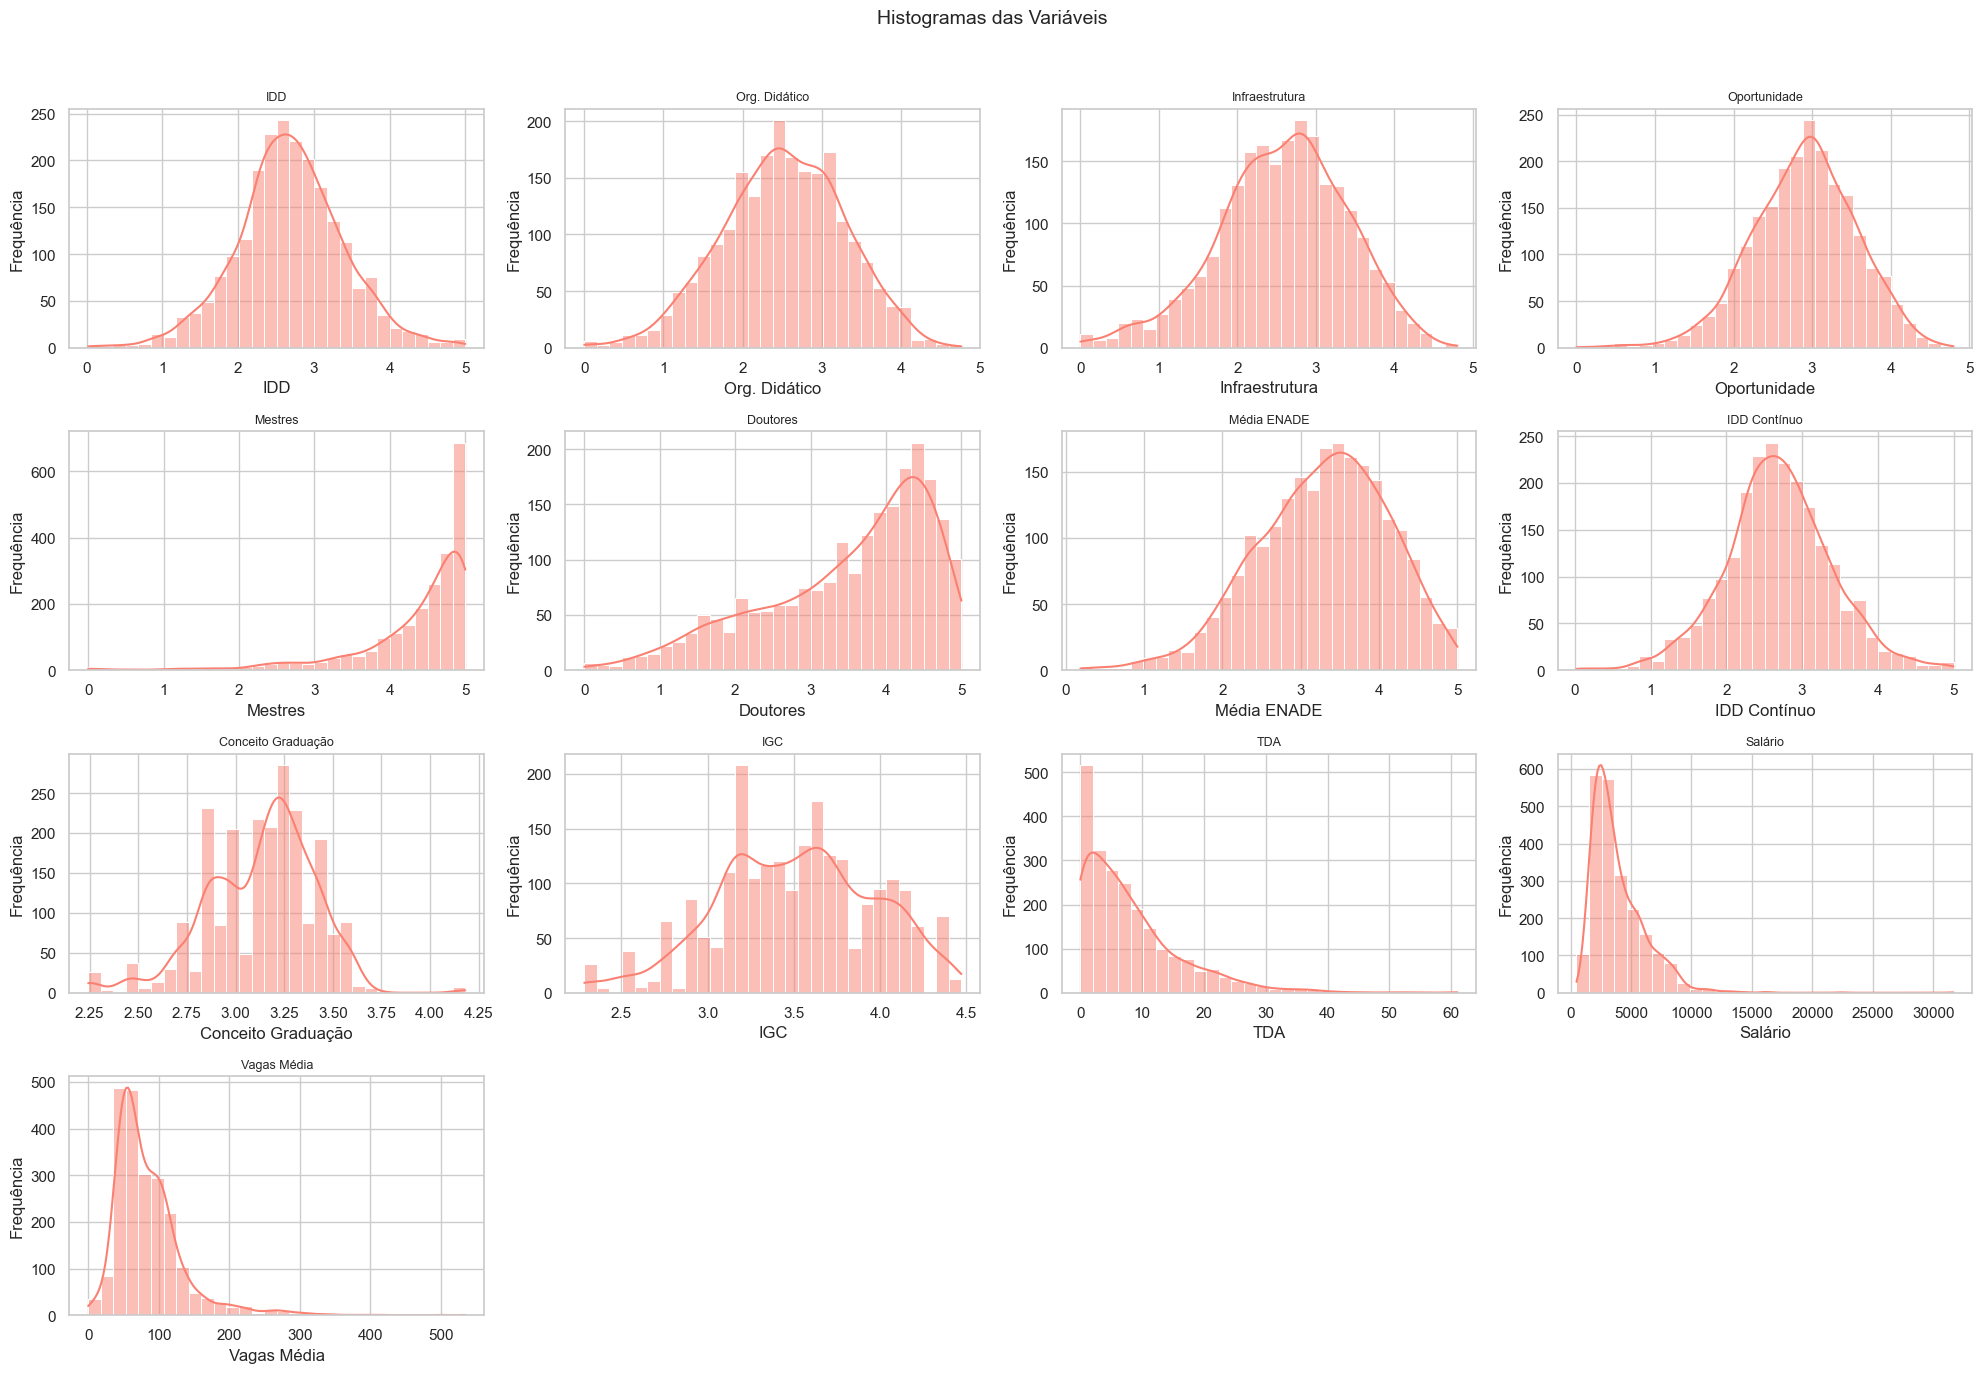
\includegraphics[width=\textwidth]{fig1_histograms.png}
    \caption*{Fonte: Elaboração própria (2025), com base em dados do INEP e RAIS (Brasil, 2018-2023).}
\end{figure}

A Figura \ref{fig:heatmaps} apresenta um mapa de calor que ilustra a distribuição das variáveis educacionais por estado, revelando nítidos padrões regionais. Nos indicadores de qualidade como IDD, organização didático-pedagógica e infraestrutura os estados das regiões Sul e Sudeste consistentemente exibem valores mais elevados. Esse padrão se repete para a qualificação docente (mestrado e doutorado) e para os conceitos do ENADE e IGC. De forma semelhante, os maiores salários médios para egressos concentram-se no Sul, Sudeste e no Distrito Federal. Curiosamente, as maiores taxas de desistência (TDA) também se destacam nos estados do Sudeste, enquanto a oferta de vagas se mostra heterogênea, com alta concentração em São Paulo e em algumas localidades da região Norte.

Essas disparidades regionais estão intrinsecamente ligadas a questões estruturais e econômicas que impactam a permanência estudantil. Estados com menor investimento em infraestrutura e qualificação docente, por exemplo, podem criar um ambiente menos propício à continuidade dos estudos. Simultaneamente, mercados de trabalho com salários mais baixos para recém-formados podem impor uma pressão socioeconômica que dificulta a retenção dos discentes. Essa pressão muitas vezes se traduz na necessidade de o estudante ingressar prematuramente no mercado de trabalho, em ocupações que não exigem qualificação superior, tornando a dedicação aos estudos insustentável. A percepção de um baixo retorno financeiro futuro sobre o investimento educacional também pode minar a motivação para a conclusão do curso.

Além desses fatores, o acesso limitado a políticas de assistência estudantil, o transporte precário e as dificuldades de moradia acentuam as desigualdades. A ausência de moradia universitária ou de auxílios-moradia, por exemplo, pode forçar o aluno a longos deslocamentos diários, consumindo tempo e energia que seriam dedicados ao aprendizado. As limitações no desenvolvimento local refletem-se diretamente nas condições de estudo, especialmente para alunos de baixa renda. Essa realidade evidencia que a desistência não pode ser analisada de forma isolada, mas sim dentro de um contexto socioeconômico e territorial mais amplo.

Dessa forma, torna-se imprescindível que as políticas públicas de permanência considerem as especificidades de cada região. Somente com ações integradas e direcionadas será possível reduzir as disparidades e promover uma educação superior mais equitativa no país. Isso implica articular políticas educacionais com estratégias de desenvolvimento local, fomentando ecossistemas de inovação que possam absorver a mão de obra qualificada. A universidade, nesse modelo, atua não apenas como formadora, mas como um motor para o progresso regional sustentável.

\begin{figure}[H]
    \centering
    \caption{Mapas de calor das variáveis do modelo por estado}
    \label{fig:heatmaps}
    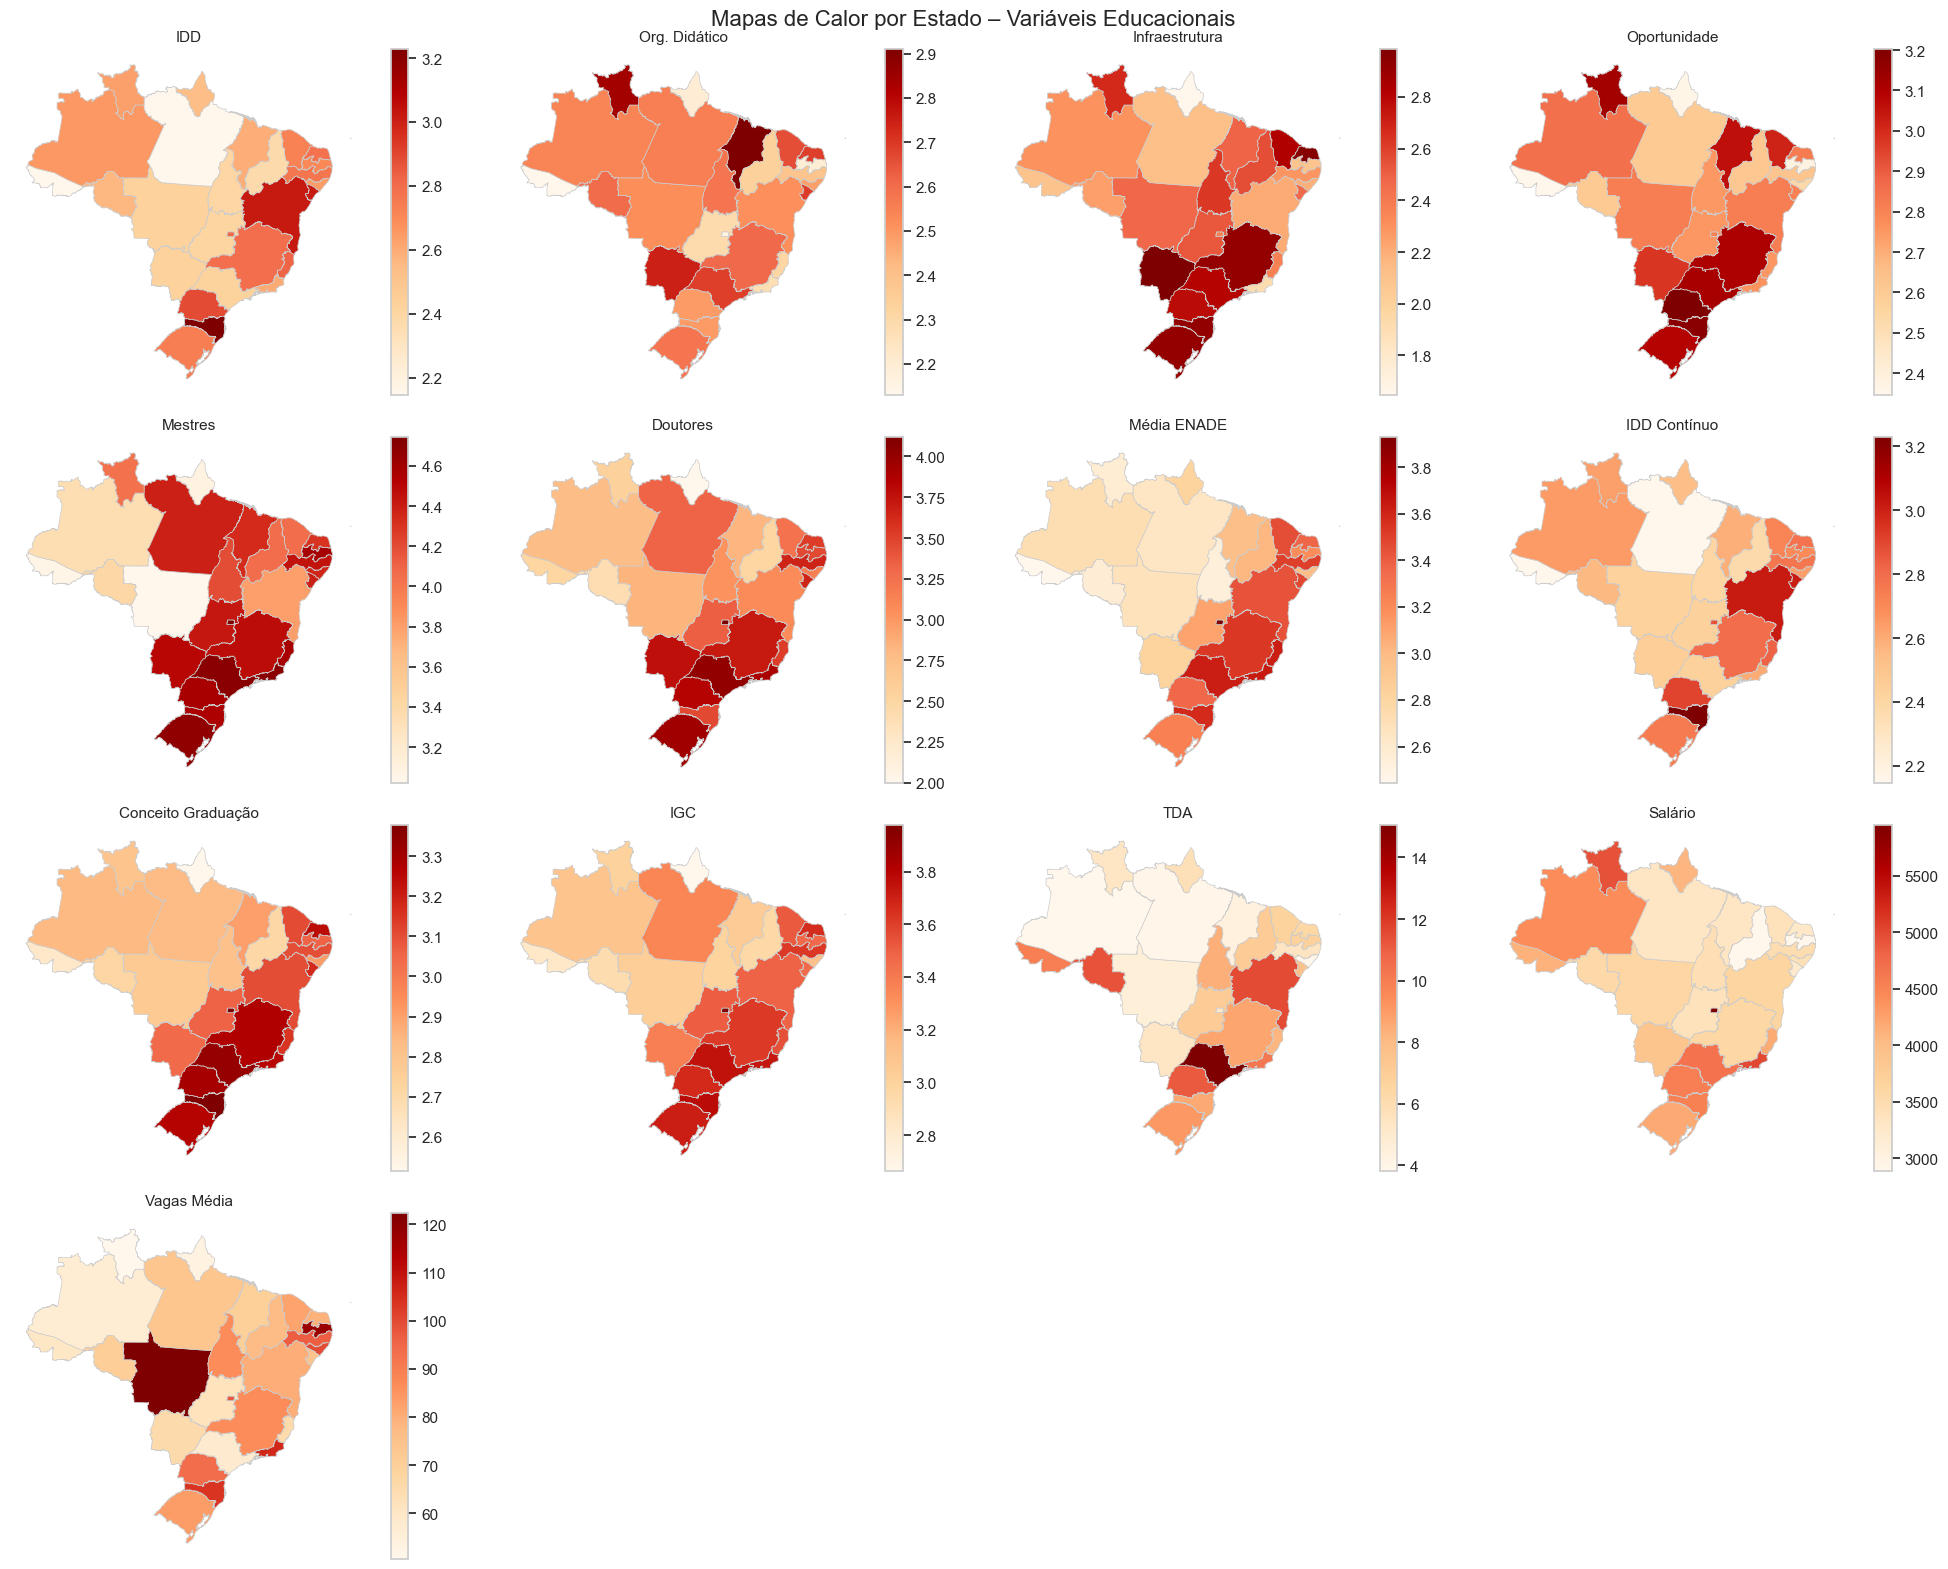
\includegraphics[width=\textwidth]{fig2_heatmaps.png}
    \caption*{Nota: Os valores correspondem à média por curso das IFES em cada estado (Brasil, 2018-2023). \\ Fonte: Elaboração própria (2025), com base em dados do INEP e da RAIS.}
\end{figure}

A Figura \ref{fig:corr} apresenta o mapa de correlação entre as variáveis do modelo. Observam-se diversas correlações positivas e fortes entre os indicadores de qualidade. A associação mais elevada (próxima de 1,0) ocorre entre o IDD padronizado e o IDD Contínuo. Relações fortes também são notadas entre o Conceito de Graduação e o IGC (0,89), e entre a Organização Didático-Pedagógica e a Infraestrutura (0,75), sugerindo que cursos bem estruturados pedagogicamente tendem a ter melhor infraestrutura. Adicionalmente, a correlação de 0,62 entre as notas do ENADE e o Conceito de Graduação indica que cursos com melhores avaliações conceituais geralmente possuem discentes com melhor desempenho.

Um resultado de destaque é a baixa correlação entre a variável dependente, a Taxa de Desistência (TDA), e cada uma das variáveis explicativas individualmente. Isso sugere que a desistência é um fenômeno complexo e multifatorial, que não pode ser adequadamente explicado por um único indicador de forma isolada. A análise conjunta de múltiplas variáveis, como a proposta pelo modelo de machine learning, torna-se, portanto, fundamental.

De modo semelhante, a variável Salário apresenta correlações baixas com os demais indicadores do modelo, que são predominantemente institucionais. Este resultado é coerente, uma vez que o salário é uma variável de natureza socioeconômica, influenciada por fatores de mercado externos à universidade, e não apenas pelos indicadores internos de qualidade dos cursos.

\begin{figure}[H]
    \centering
    \caption{Matriz de correlação de Pearson entre as variáveis do modelo}
    \label{fig:corr}
    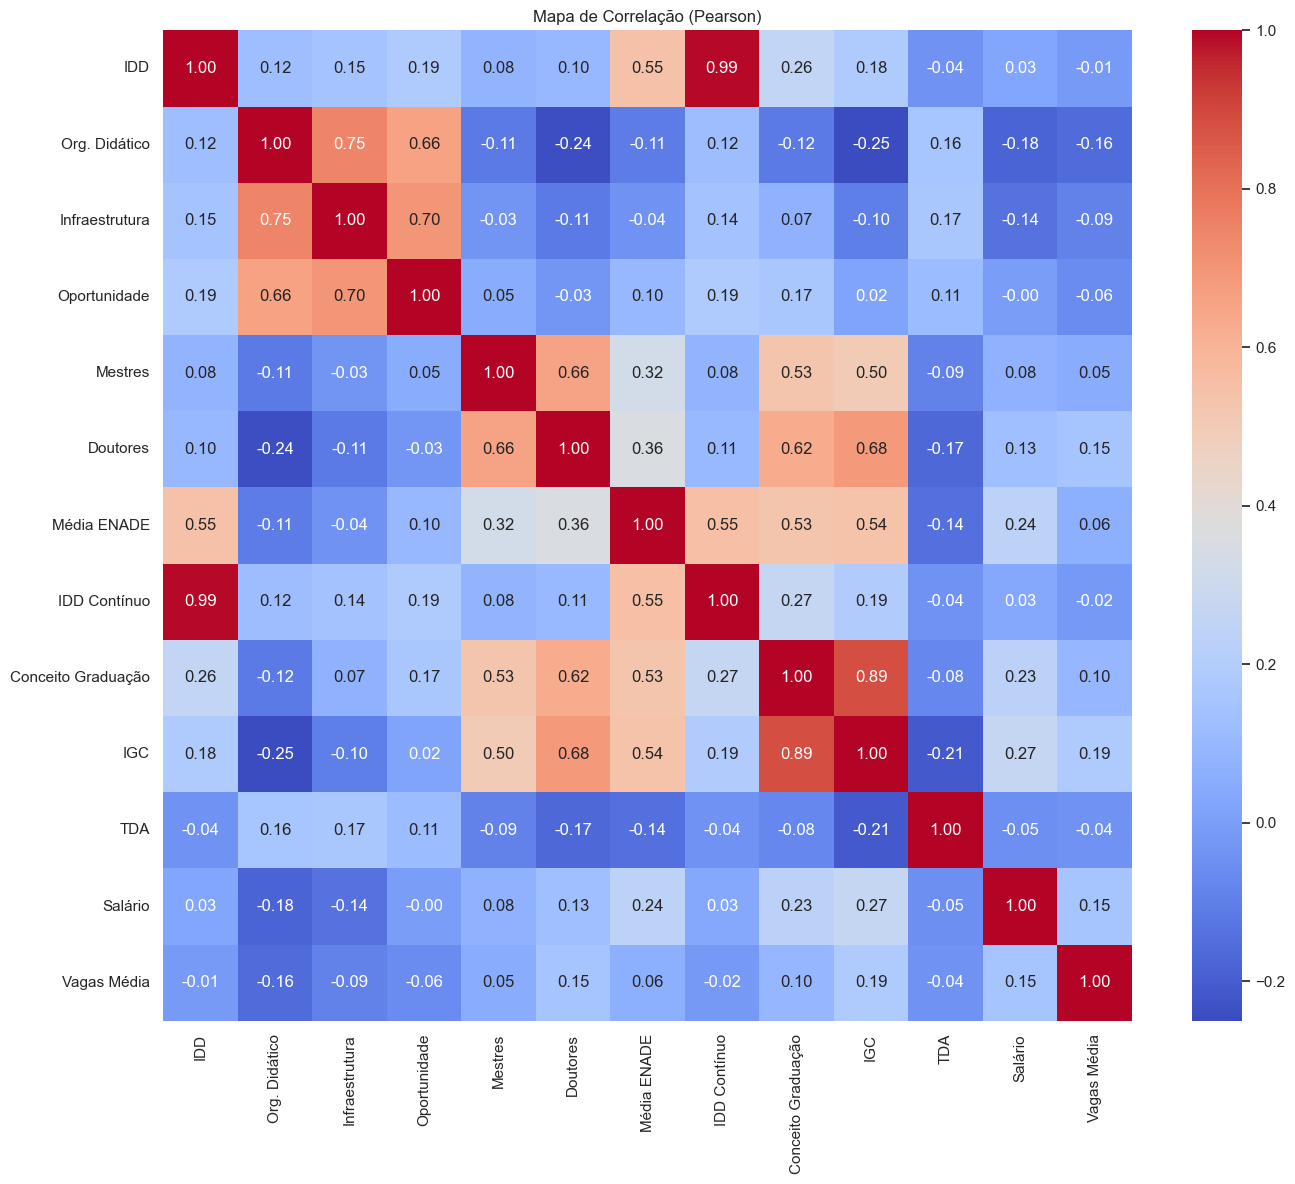
\includegraphics[width=0.8\textwidth]{fig3_correlation.png}
    \caption*{Nota: As correlações foram calculadas a partir dos valores médios por curso das IFES (Brasil, 2018-2023). \\ Fonte: Elaboração própria (2025), com base em dados do INEP e da RAIS.}
\end{figure}

A Figura \ref{fig:scatter} exibe os gráficos de dispersão entre a variável dependente Taxa de Desistência Acumulada (TDA), no eixo y e cada uma das variáveis explicativas, no eixo x. A análise visual desses gráficos permite identificar diferentes tipos de associação entre as variáveis.

Para diversas variáveis, não se observa uma relação linear clara. É o caso da relação entre a TDA e os indicadores IDD, Organização Didático-Pedagógica e as notas de titulação do corpo docente (mestrado e doutorado). Nesses gráficos, os pontos se encontram amplamente dispersos, sem uma tendência positiva ou negativa definida.

Em contrapartida, alguns indicadores sugerem uma relação negativa, ainda que fraca, com a desistência. Cursos com melhores notas de infraestrutura e de oportunidade de ampliação da formação, por exemplo, tendem a concentrar as taxas de desistência em níveis mais baixos. De forma semelhante, cursos com maiores conceitos no ENADE, no Conceito de Graduação (CPC) e no IGC também parecem estar associados a menores taxas de desistência.

Finalmente, a relação entre a TDA e a oferta de vagas indica uma associação positiva: instituições que ofertam um número maior de vagas tendem a registrar também maiores taxas de desistência estudantil.

\begin{figure}[H]
    \centering
    \caption{Gráficos de dispersão entre a Taxa de Desistência (TDA) e as variáveis explicativas}
    \label{fig:scatter}
    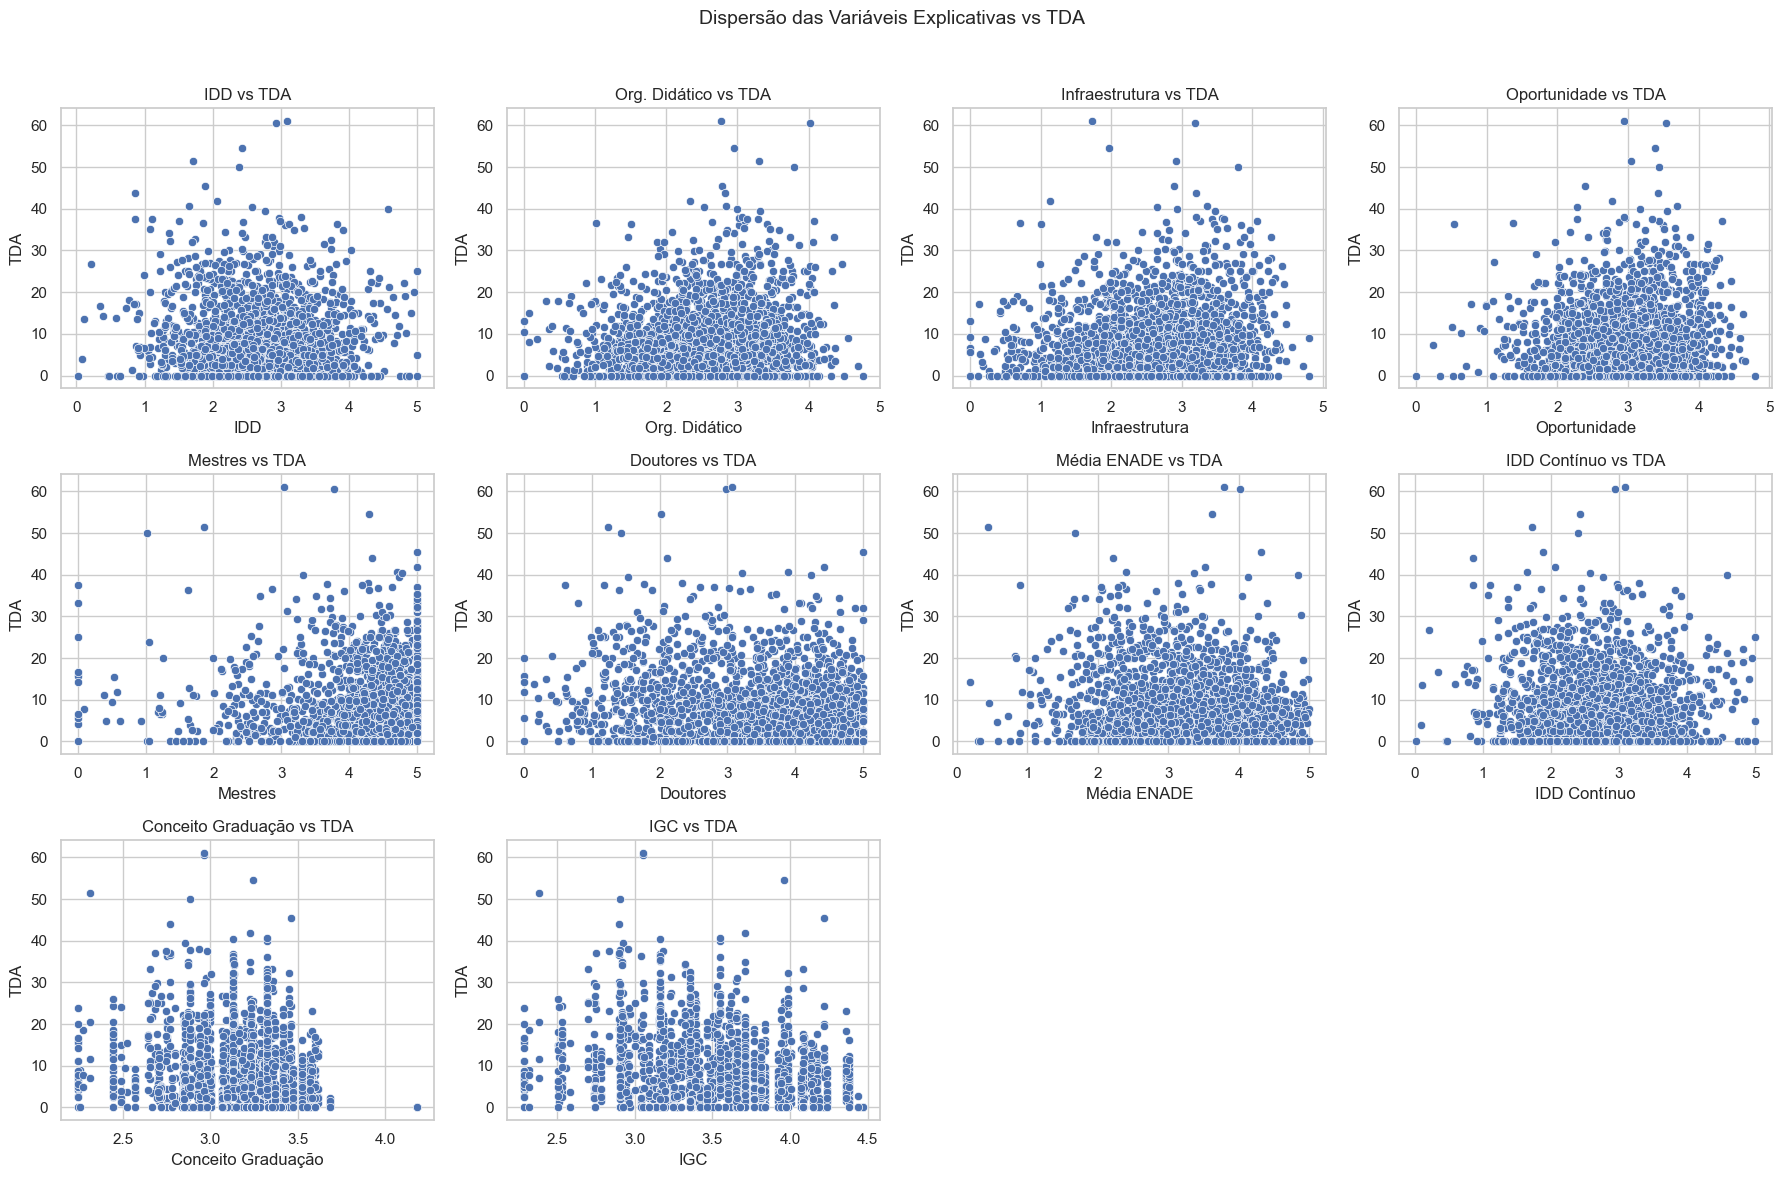
\includegraphics[width=\textwidth]{fig4_scatter.png}
    \caption*{Nota: As variáveis foram agregadas como média por curso das IFES (Brasil, 2018-2023). \\ Fonte: Elaboração própria (2025), com base em dados do INEP e da RAIS.}
\end{figure}

Conforme observado na análise descritiva, muitas das variáveis não apresentam uma relação linear clara com a taxa de desistência estudantil. Este fato reforça a hipótese de que a desistência é um fenômeno complexo, influenciado pela interação de múltiplos fatores que agem de forma combinada.

Tal complexidade justifica a aplicação de um modelo não linear, capaz de capturar essas interações. Portanto, este trabalho emprega o algoritmo Random Forest, via Machine Learning, para identificar os padrões de relacionamento entre o conjunto de variáveis explicativas e a variável dependente.

A seção seguinte apresentará a análise e as considerações sobre os resultados obtidos com o modelo proposto.


% --- CAPÍTULO MANUAL: Discussão dos Resultados ---
\refstepcounter{manualchapter}
\addcontentsline{toc}{chapter}{\protect\numberline{\themanualchapter}Discussão dos Resultados}
\vspace{2em}
\noindent\textbf{\themanualchapter. Discussão dos Resultados}
\vspace{1em}
\par

A Tabela 02 apresenta o relatório de classificação do modelo Random Forest, detalhando as métricas de performance para cada classe e os resultados gerais. Conforme a metodologia adotada, a variável contínua TDA (Taxa de Desistência Acumulada) foi convertida em binária usando a mediana como ponto de corte: a Classe 0 representa uma baixa taxa de desistência (valores abaixo da mediana) e a Classe 1, uma alta taxa de desistência (valores acima da mediana). O modelo foi treinado com 70\% dos dados e testado com os 30\% restantes.

A análise da Classe 0 (Baixa Desistência) revela uma precisão de 0,73, o que significa que, das vezes em que o modelo previu um curso como sendo de baixa desistência, ele acertou em 73\% dos casos. O recall de 0,70 indica que o modelo identificou corretamente 70\% de todos os cursos que verdadeiramente pertenciam a essa classe. O F1-Score, que pondera essas duas métricas, foi de 0,71, demonstrando um bom equilíbrio.

Para a Classe 1 (Alta Desistência), a precisão foi de 0,71, indicando que 71\% das previsões de alta desistência estavam corretas. O recall de 0,74 demonstra a capacidade do modelo de identificar corretamente 74\% de todos os casos reais de alta desistência. O F1-Score de 0,72 confirma a consistência entre precisão e recall também para esta classe.

A acurácia geral do modelo foi de 0,72, significando que 72\% das previsões totais foram corretas, um desempenho robusto que, porém, pode ser aprimorado com a inclusão de novas variáveis. É fundamental notar que a métrica de suporte (support) está bem balanceada entre as classes (221 para a classe 0 e 220 para a classe 1). Esse equilíbrio, resultante do uso da mediana para a divisão dos dados, é crucial para evitar vieses e garantir a confiabilidade das métricas de performance avaliadas.

\begin{table}[H]
    \centering
    \caption{Relatório de classificação do modelo Random Forest para predição da desistência}
    \label{tab:class_report}

    % Espaçamento e alinhamento ajustados
    \renewcommand{\arraystretch}{1.2}
    \setlength{\tabcolsep}{5pt}

    \begin{tabular}{%
        p{3.5cm}  % Nome da métrica ou classe
        >{\centering\arraybackslash}p{2.7cm}  % Precision
        >{\centering\arraybackslash}p{2.7cm}  % Recall
        >{\centering\arraybackslash}p{2.7cm}  % F1-score
        >{\centering\arraybackslash}p{2.7cm}  % Support
    }

        \toprule
        & \textbf{Precision} & \textbf{Recall} & \textbf{F1-score} & \textbf{Support} \\
        \midrule
        Classe: 0 & 0.73 & 0.70 & 0.71 & 221 \\
        Classe: 1 & 0.71 & 0.74 & 0.72 & 220 \\
        \midrule
        \textbf{Accuracy} & -- & -- & 0.72 & 441 \\
        \textbf{Macro avg} & 0.72 & 0.72 & 0.72 & 441 \\
        \textbf{Weighted avg} & 0.72 & 0.72 & 0.72 & 441 \\
        \bottomrule
    \end{tabular}

    \caption*{\textit{Fonte}: Elaboração própria (2025).}
\end{table}


A Figura \ref{fig:conf_matrix} exibe a matriz de confusão, que visualiza o desempenho do modelo ao comparar as classes preditas com as classes reais, detalhando as métricas da Tabela \ref{tab:class_report}. A análise da matriz evidencia a principal força do modelo: sua alta capacidade de identificar corretamente os cursos com elevada taxa de desistência (Classe 1).

Essa capacidade é quantificada pelo recall (ou sensibilidade) de 0,74 para essa classe, indicando que o modelo acerta na identificação de 74\% de todos os cursos que de fato apresentam problemas graves de desistência. Essa característica é de grande valor prático, pois permite que gestores e formuladores de políticas públicas direcionem recursos e atenção prioritária às instituições que mais necessitam de intervenção.

Complementarmente, a taxa de Falsos Negativos é de 0,26 (1-0,74), um valor relativamente baixo que demonstra que o modelo raramente deixa de identificar um caso crítico. Somado aos valores de precisão e F1-Score, todos superiores a 0,70, o bom desempenho do recall para a classe de maior interesse confirma que o modelo é robusto e bem balanceado.

\begin{figure}[H]
    \centering
    \caption{Matriz de confusão normalizada do modelo Random Forest para as classes de desistência}
    \label{fig:conf_matrix}
    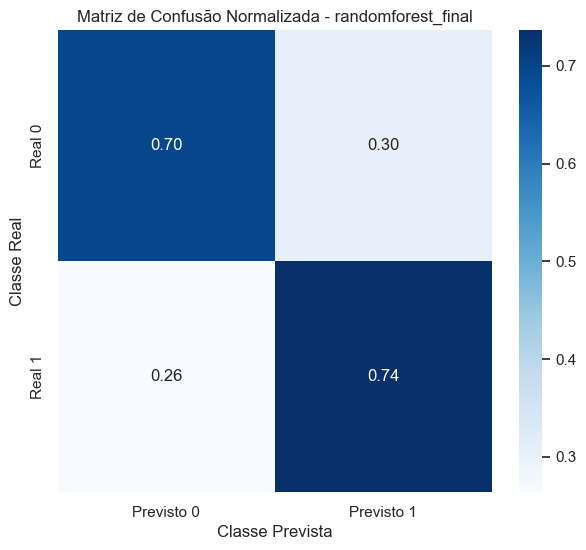
\includegraphics[width=0.7\textwidth]{fig5_confusion_matrix.png}
    \caption*{Fonte: Elaboração própria (2025).}
\end{figure}

A Figura \ref{fig:feat_imp} exibe a importância de cada variável (feature importance) na construção do modelo Random Forest, ranqueando os fatores de acordo com seu poder preditivo sobre a taxa de desistência. A análise da hierarquia revela que a qualidade institucional é o fator predominante. O Índice Geral de Cursos (IGC) destacou-se como a variável mais influente, seguido de perto pelo Conceito de Graduação (CPC), o que reforça que cursos e instituições com piores avaliações estão consistentemente associados a maiores taxas de abandono.
Logo após, a oferta de vagas surge como um fator relevante, indicando que cursos com um número maior de vagas tendem a ter desistência mais elevada, possivelmente devido a critérios de seleção menos rigorosos. A qualificação docente e fatores socioeconômicos também se mostraram importantes: a titulação de doutorado impacta positivamente na permanência, enquanto baixos salários de mercado para a área de formação se associam a uma maior desistência. Outras variáveis, como Conceito ENADE e Infraestrutura, seguem a mesma lógica, embora com impacto progressivamente menor.

A análise de importância revela que fatores institucionais (como IGC e CPC), socioeconômicos (como o salário) e estruturais (como infraestrutura e qualificação docente) têm uma contribuição significativamente maior para explicar a desistência do que o desempenho discente medido pelo IDD, que apresentou um dos menores pesos. Isso indica que investimentos na melhora de indicadores de qualidade institucional, como a infraestrutura, o corpo docente e a adoção de melhores práticas pedagógicas, podem ter um impacto direto na redução das taxas de desistência.

Adicionalmente, como o fator salarial demonstra forte influência, políticas de permanência que fortaleçam a perspectiva de carreira dos estudantes — como a oferta de programas de estágio, projetos de empreendedorismo e o fomento à inserção no mercado de trabalho — são estratégias cruciais para aumentar a retenção discente.

\begin{figure}[H]
    \centering
    \caption{Importância das variáveis (feature importance) no modelo Random Forest}
    \label{fig:feat_imp}
    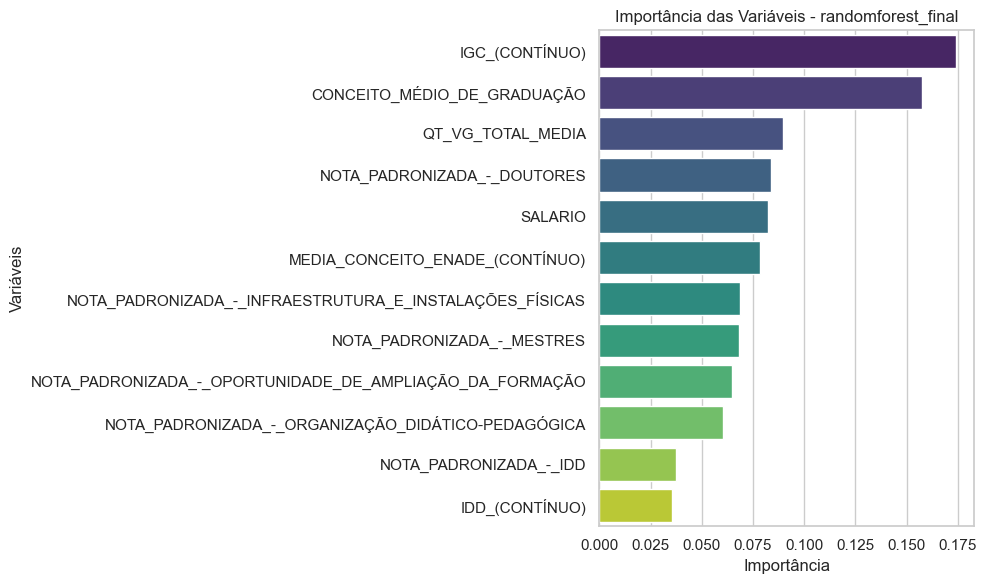
\includegraphics[width=\textwidth]{fig6_feature_importance.png}
    \caption*{Fonte: Elaboração própria (2025).}
\end{figure}

A Figura \ref{fig:perf_curves} exibe as curvas de performance do modelo, especificamente a curva ROC e a curva de precisão-revocação, que permitem uma avaliação visual de sua capacidade preditiva.

A análise da curva ROC (Receiver Operating Characteristic) revela uma Área Sob a Curva (AUC) de 0,795. Este valor indica uma boa capacidade de discriminação, significando que há 79,5\% de probabilidade de o modelo atribuir uma pontuação de risco maior a um caso positivo (alta desistência) do que a um caso negativo (baixa desistência) escolhido aleatoriamente. Adicionalmente, o fato de a curva se manter consistentemente acima da linha de referência diagonal atesta o bom desempenho do modelo em comparação a um classificador aleatório.

A curva de precisão-revocação, por sua vez, apresenta uma Precisão Média (Average Precision - AP) de 0,772, confirmando a robustez do modelo. Observa-se que o modelo consegue manter uma precisão superior a 0,75 para níveis de revocação de até 0,6. A queda na precisão em níveis mais altos de revocação é um comportamento esperado, pois, para identificar a totalidade dos casos positivos (revocação próxima de 1,0), o modelo inevitavelmente passa a classificar incorretamente alguns casos negativos, o que demonstra o clássico trade-off entre as duas métricas.

\begin{figure}[H]
    \centering
    \caption{Curvas de performance do modelo: ROC/AUC e Precisão-Revocação}
    \label{fig:perf_curves}
    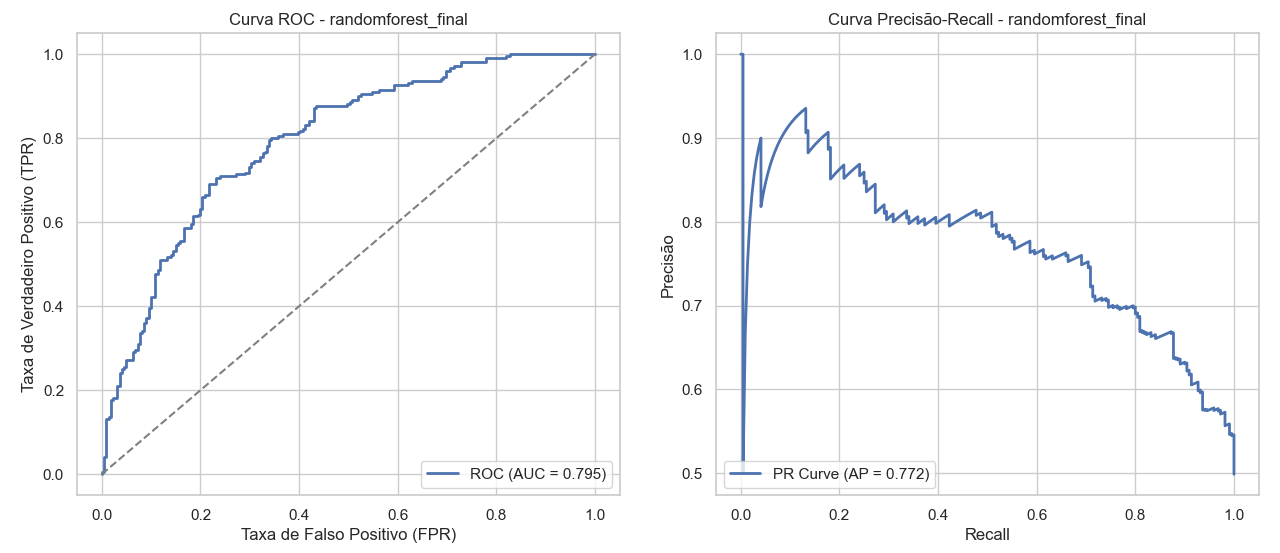
\includegraphics[width=\textwidth]{fig7_performance_curves.png}
    \caption*{Fonte: Elaboração própria (2025).}
\end{figure}

A Figura \ref{fig:diag_plots} apresenta os gráficos de calibração e de distribuição das probabilidades, que complementam a análise de performance do modelo.

No gráfico de calibração, observa-se que a curva do modelo (linha laranja) acompanha de perto a linha tracejada, que representa a calibração perfeita. Apesar de pequenas oscilações, essa proximidade indica que as probabilidades geradas pelo modelo são confiáveis, ou seja, uma predição de 70\% de chance de desistência corresponde, na prática, a uma ocorrência real de aproximadamente 70\%.

O gráfico de distribuição das probabilidades, por sua vez, demonstra a boa capacidade de separação entre as classes. As predições para a Classe 0 (Baixa Desistência) concentram-se majoritariamente na faixa de 0,2 a 0,5, enquanto as da Classe 1 (Alta Desistência) apresentam picos entre $0,6\text{ e }0,8$. A zona de sobreposição, principalmente no intervalo entre $0,4\text{ e }0,6$, representa os casos de maior incerteza. É nessa faixa que se encontram os exemplos mais difíceis de classificar, o que justifica os erros de predição detalhados na matriz de confusão.

\begin{figure}[H]
    \centering
    \caption{Gráficos de diagnóstico do modelo: curva de calibração e distribuição de probabilidades}
    \label{fig:diag_plots}
    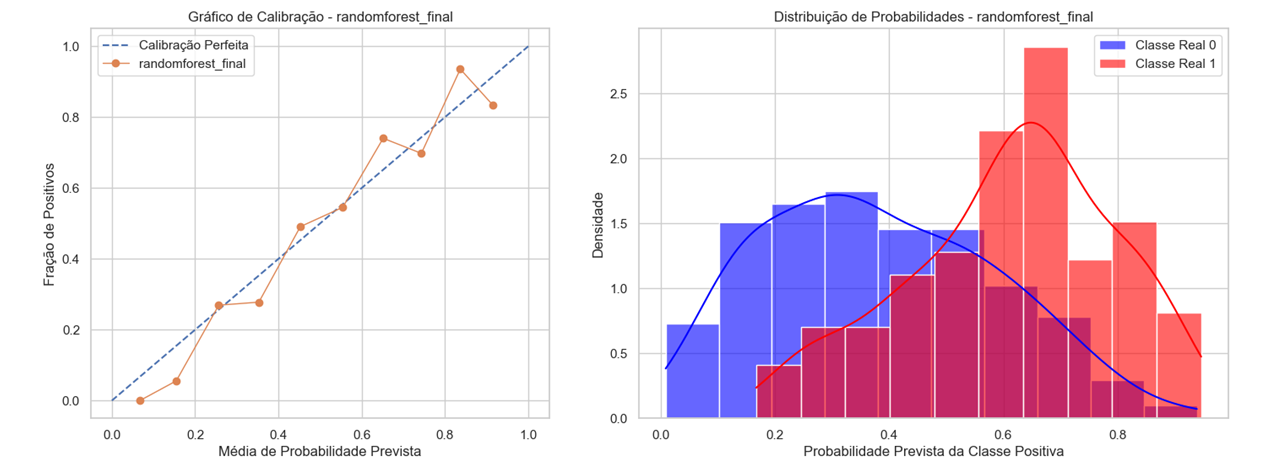
\includegraphics[width=\textwidth]{fig8_diagnostic_plots.png}
    \caption*{Fonte: Elaboração própria (2025).}
\end{figure}

A Figura \ref{fig:residuals} exibe os gráficos de diagnóstico baseados nos resíduos do modelo. No primeiro gráfico, que plota os resíduos padronizados, observa-se uma distribuição aleatória dos pontos em torno da linha horizontal em zero. A ausência de padrões claros (como um formato de cone, que indicaria heterocedasticidade) sugere que o modelo não possui viés sistemático. Adicionalmente, como a maior parte dos resíduos se encontra dentro dos limites de confiança (linhas tracejadas), o conjunto desses fatores atesta o bom ajuste do modelo.

O segundo gráfico, que compara os resíduos com as probabilidades preditas, também confirma o bom funcionamento do modelo para uma tarefa de classificação. O padrão esperado nesse caso é a formação de dois "feixes" de resíduos, o que é claramente visível na figura. A banda inferior corresponde aos casos da Classe 0 (Baixa Desistência), que recebem probabilidades mais baixas e, portanto, geram resíduos negativos. A banda superior representa os casos da Classe 1 (Alta Desistência), que recebem probabilidades mais altas e resultam em resíduos positivos. A nítida separação dessas duas bandas, sem dispersões irregulares, indica que o modelo está atribuindo probabilidades de forma coerente com as classes verdadeiras, reforçando a validade do ajuste.


\begin{figure}[H]
    \centering
    \caption{Gráficos de análise de resíduos do modelo}
    \label{fig:residuals}
    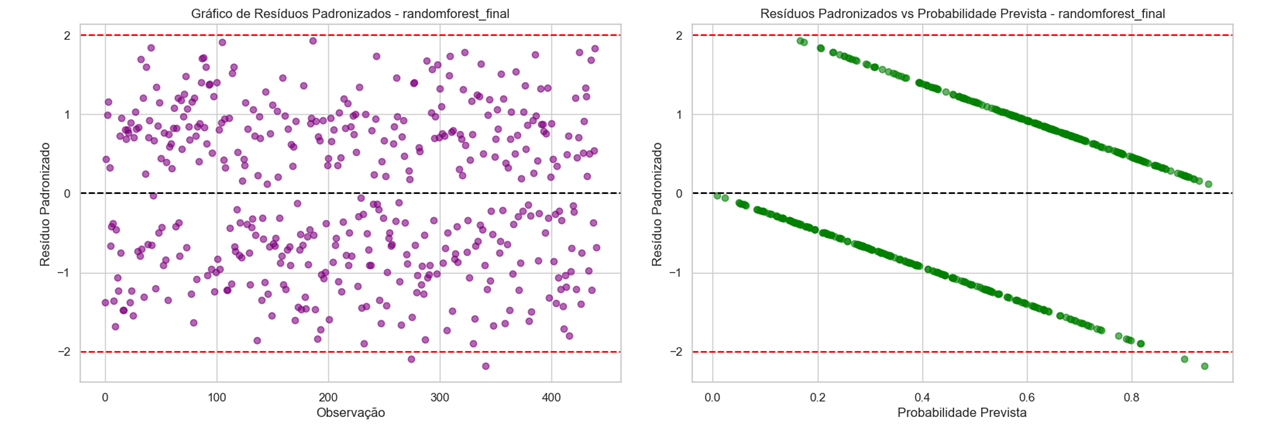
\includegraphics[width=\textwidth]{fig9_residuals.png}
    \caption*{Fonte: Elaboração própria (2025).}
\end{figure}

A seção a seguir apresenta as considerações finais deste estudo. Nela, serão discutidas tanto as contribuições do trabalho para o âmbito acadêmico quanto as suas principais limitações, além de sugestões para pesquisas futuras.


% --- CAPÍTULO MANUAL: Considerações Finais ---
\refstepcounter{manualchapter}
\addcontentsline{toc}{chapter}{\protect\numberline{\themanualchapter}Considerações Finais}
\vspace{2em}
\noindent\textbf{\themanualchapter. Considerações Finais}
\vspace{1em}
\par

Este estudo analisou a desistência nos cursos de graduação das Instituições Federais de Ensino Superior (IFES) no Brasil, durante o período de 2018 a 2023, a partir da integração de dados educacionais (INEP) e laborais (RAIS) com a aplicação de técnicas de machine learning. Por meio do modelo Random Forest, foi possível identificar os fatores que mais influenciam a Taxa de Desistência Acumulada (TDA) e construir uma ferramenta preditiva com elevada capacidade discriminativa.

Os resultados apontam que variáveis institucionais como o Índice Geral de Cursos (IGC), o Conceito Preliminar de Curso (CPC) e a quantidade de vagas ofertadas estão entre os principais preditores da desistência. Em seguida, destacam-se características acadêmicas como a titulação do corpo docente, a infraestrutura e o desempenho em indicadores como ENADE e IDD. Adicionalmente, a variável associada ao salário médio dos egressos surge como um fator relevante, ressaltando a conexão entre expectativas econômicas e a permanência discente.

O desempenho do modelo foi robusto, com uma Área Sob a Curva ROC (AUC) de 0,795 e uma Precisão Média (Average Precision) de 0,772, indicando boa capacidade de generalização. A matriz de confusão revelou equilíbrio na classificação, e os diagnósticos de calibração, distribuição de probabilidades e análise de resíduos confirmaram a coerência e a validade do modelo, sem a presença de vieses sistemáticos.

Do ponto de vista acadêmico, este trabalho contribui ao aplicar uma abordagem preditiva de machine learning na análise da desistência, complementando os modelos explicativos tradicionais. Do ponto de vista social, os resultados oferecem subsídios para que gestores e formuladores de políticas públicas identifiquem cursos com maior vulnerabilidade, permitindo a criação de estratégias preventivas e a alocação mais eficiente de recursos.

Por fim, este estudo reforça a necessidade de políticas de permanência integradas, que considerem não apenas os indicadores institucionais, mas também o impacto das expectativas de carreira e do mercado de trabalho na trajetória dos estudantes. A ampliação deste modelo, com a inclusão de outras variáveis socioeconômicas e psicossociais, representa uma perspectiva promissora para pesquisas futuras.

% --- REFERÊNCIAS MANUAL: Referências ---
\postextual
\bibliography{referencias}
\end{document}
